\begin{figure}[htbp]
\centering
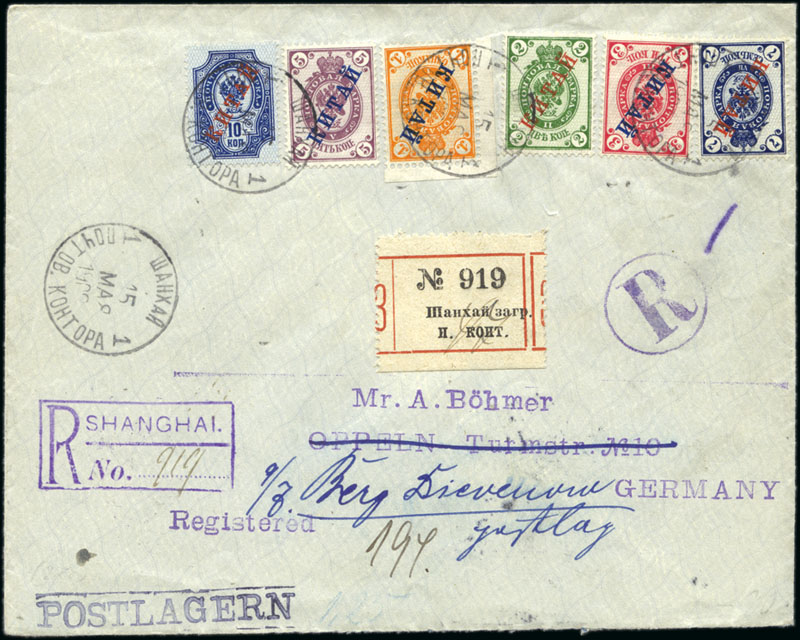
\includegraphics[width=.95\textwidth]{../russian-post-offices-in-china/10056.jpg}
\caption{
10056 SHANGHAI: 1902 Cover registered to Germany with "KITAI" 1k, 2k, 3k, 5k, 
7k and 10k tied by Shanghai 15.05.02 cds (T\&S type 2), paying triple rate 
plus registration, with boxed registered cachet and reg'd label adjacent, 
and amended 'R', "POSTLAGERN" (Poste Restante) hs and Oppeln and Berg-Dievenow 
bs on arrival, very colourful franking
\euro 400.00
}  
\end{figure} 

\begin{figure}[htbp]
\centering
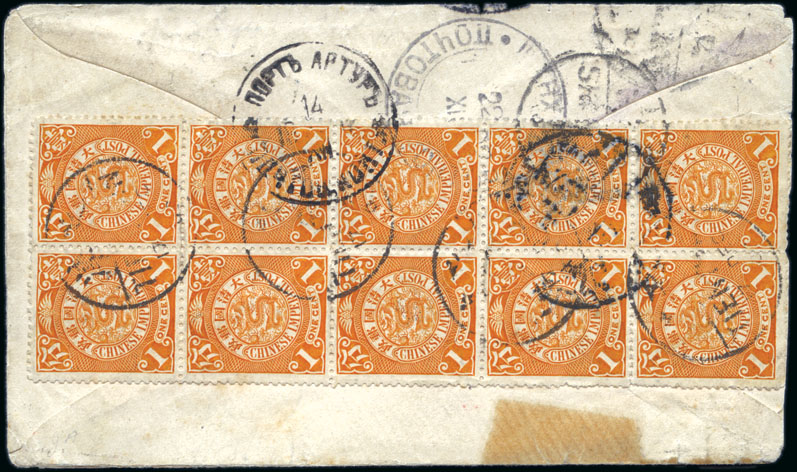
\includegraphics[width=.95\textwidth]{../russian-post-offices-in-china/10057.jpg}
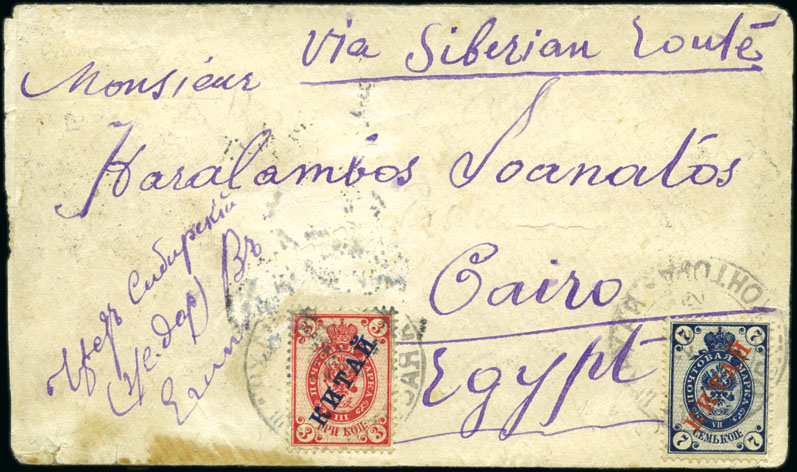
\includegraphics[width=.95\textwidth]{../russian-post-offices-in-china/10057-1.jpg}
\caption{
 10057	SHANGHAI: 1902 Cover to Egypt, endorsed via "Siberian route" in English 
 \& Russian, franked on the reverse with China block of ten 1c Dragons with 
 Tientsin 17.12.02 cds, sent to Shanghai where it was passed to the Russian 
 P.O. and franked with "KITAI" 3k and 7k tied by Shanghai 22.12.02 cds (T\&S type 1), 
 Port Arthur bs, adhesive stain at foot, a rare destination and superb franking
\euro 600.00
}  
\end{figure} 

\begin{figure}[htbp]
\centering
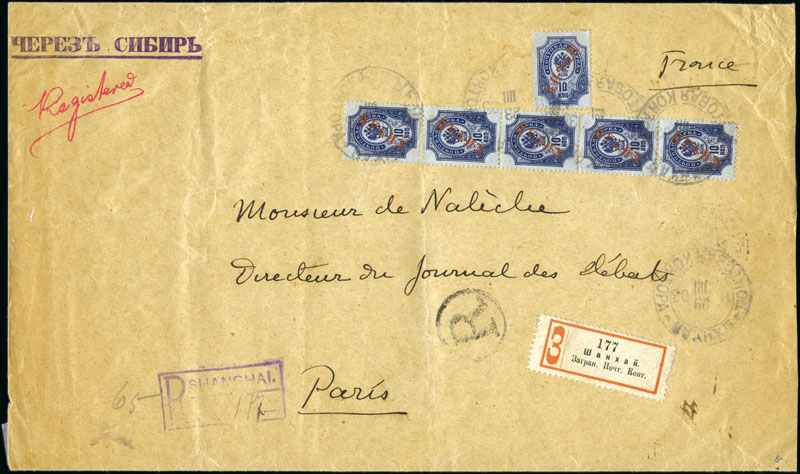
\includegraphics[width=.95\textwidth]{../russian-post-offices-in-china/10058.jpg}
\caption{
10058	SHANGHAI: 1903 Cover registered to France with "KITAI" 10k 
in vertical strip of five and single, paying four times the 10k rate plus reg'n 
fee, tied by Shanghai 23.04.03 cds (T\&S type 1, Gregorian calendar), 
Shanghai boxed reg'n hs and reg'd label, sent via Port Arthur (T\&S type 1 and 2 bs) 
for conveyance on Chinese Eastern Railway, Moscow and Paris bs, central fold, 
scarce high rate
\euro 700.00. 
}  
\end{figure} 

\begin{figure}[htbp]
\centering
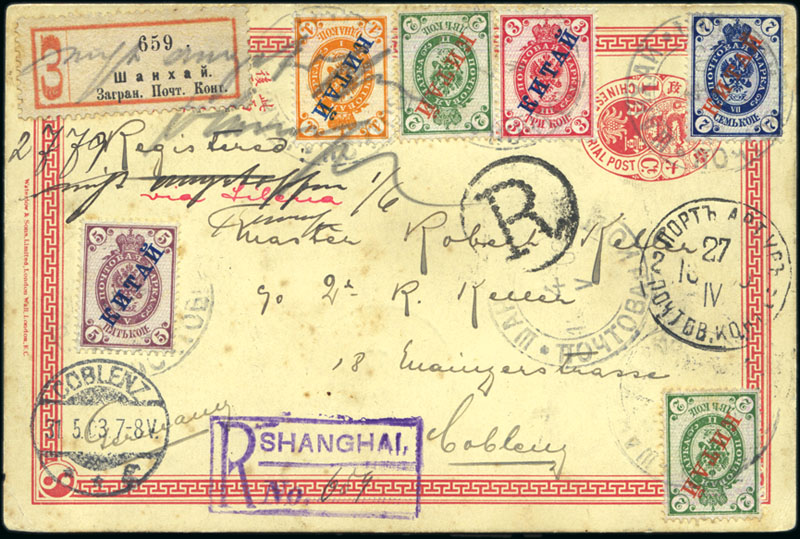
\includegraphics[width=.95\textwidth]{../russian-post-offices-in-china/10059.jpg}
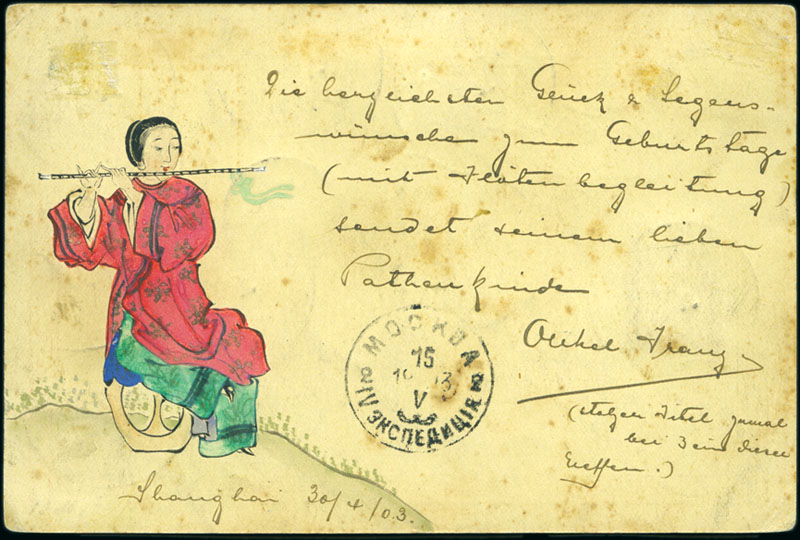
\includegraphics[width=.95\textwidth]{../russian-post-offices-in-china/10059-1.jpg}
\caption{
10059	SHANGHAI: 1903 Chinese 1c postal stationery card registered to Germany, 
with "KITAI" 1k, 2k (2), 3k, 5k and 7k tied by Shanghai 4.5.03 cds (T\&S type 1, 
Gregorian calendar), with Shanghai reg'd label, boxed hs and encircled "dotted R", 
with Port Arthur, Moscow and Coblenz cds, minor soiling, hand painted decoration 
on reverse, attractive
\euro 300.00  
}  
\end{figure} 








                                                                          